\documentclass{beamer}

\usepackage[utf8]{inputenc}
\usepackage{polski}
\usepackage{beamerthemeshadow}
\begin{document}
\title{Automatic Mutual Exclusion}  
\author{Filip Rachwalak}
\date{\today} 

\frame{\titlepage}  

\frame{\frametitle{Spis treści}\tableofcontents} 

%%%%%%%%%%%%%%%%%%%%%%%%%% WSTĘP %%%%%%%%%%%%%%%%%%%%%%%%%%%

\section{Wstęp}

\subsection{Dlaczego nie mutexy?}
\frame{\frametitle{Dlaczego nie mutexy?}
\begin{block}{}
\begin{itemize}
	\item Częste i łatwe do popełnienia błędy programistów: zakleszczenia, zawieszenie GUI.  
	\item Konieczność przestrzegania kolejności zajmowanych zamków.  
	\item Im większy projekt, tym (znacznie) trudniejsze programowanie.
\end{itemize}
\end{block}
}

\subsection{Dlaczego nie pamięć transakcyjna?}
\frame{\frametitle{Dlaczego nie pamięć transakcyjna?}
\begin{block}{}
\begin{itemize}
	\item Wciąż wymaga decyzji programisty, które bloki kodu muszą być chronione.  
	\item Gry programista chce zawęzić zasięg bloku chronionego musi usunąć żądaną część kodu z bloku, a to wpływa na zrozumienie kodu np. przez następnego programistę (szczególnie w dużych projektach).
\end{itemize}
\end{block}
}

\subsection{Główna idea AME}
\frame{\frametitle{Główna idea AME}
\begin{block}{W aplikacji wielowątkowej:}
\begin{itemize}
	\item Domyślnie chroniony cały kod, deklarowanie kodu niechronionego.  
	\item Poprawność ponad wydajnością.  
	\item Łatwe zarządzanie kodem.
\end{itemize}
\end{block}
}

%%%%%%%%%%%%%%%% METODY ASYNCHRONICZNE %%%%%%%%%%%%%%%%%%%%

\section{Podstawowy model} 
\frame{\frametitle{}
\begin{center}
	\Large{\textbf{PODSTAWOWY MODEL \\ SYSTEMU AME}}
\end{center}
}

\subsection{Asynchroniczne wywołania metod}
\frame{\frametitle{Asynchroniczne wywołania metod}
\begin{block}{Automatic Mutual Exclusion:}
\begin{itemize}
	\item składa się z wywołań metod asynchronicznych,  
	\item gwarantuje, że wynik wykonanych wywołań będzie równoważny wynikowi, który byłby osiągnięty poprzez wykonanie sekwencyjne (atomowość, niekoniecznie kolejność),  
	\item kończy się, gdy wszystkie asynchroniczne metody zostaną wykonane,  
	\item osiąga współbieżność poprzez wykonywanie wywołań niekonfliktowych.
\end{itemize}
\end{block}
}

\frame{\frametitle{Działanie programu}
\begin{figure}[h]
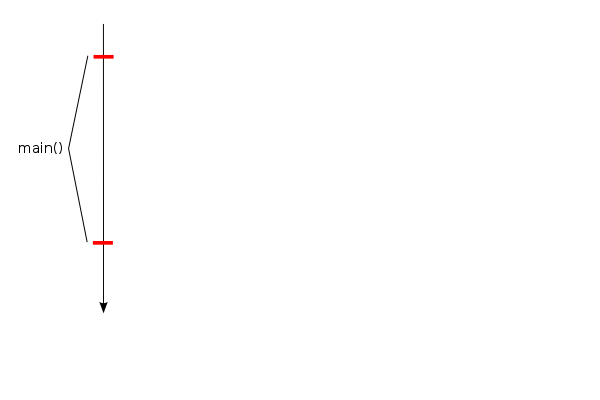
\includegraphics[scale=0.5]{figures/Rysunek1.png}
\end{figure}
}

\frame{\frametitle{Działanie programu}
\begin{figure}[h]
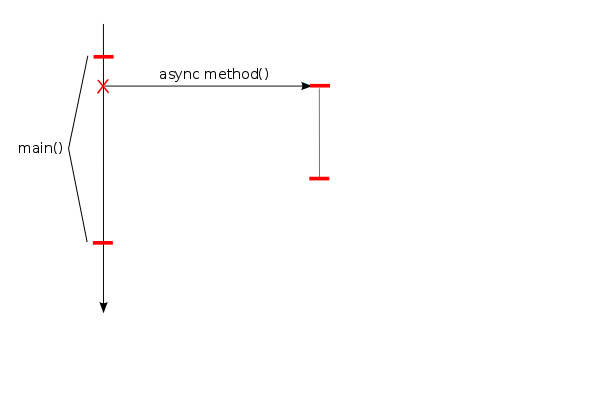
\includegraphics[scale=0.5]{figures/Rysunek2.png}
\end{figure}
}

\frame{\frametitle{Działanie programu}
\begin{figure}[h]
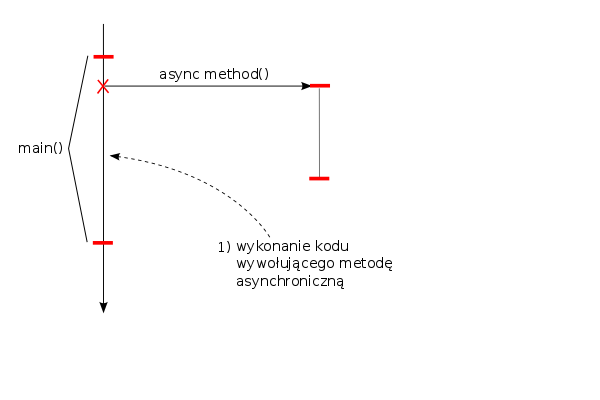
\includegraphics[scale=0.5]{figures/Rysunek3.png}
\end{figure}
}

\frame{\frametitle{Działanie programu}
\begin{figure}[h]
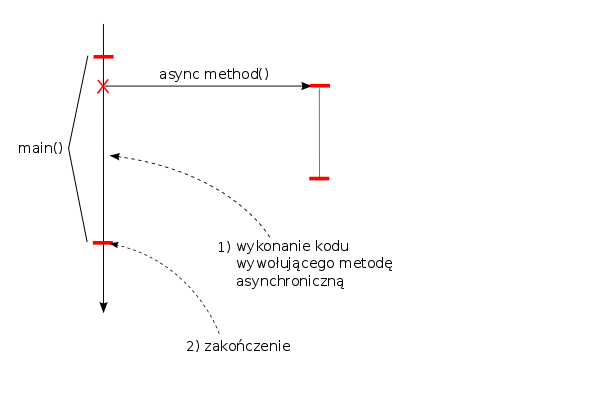
\includegraphics[scale=0.5]{figures/Rysunek4.png}
\end{figure}
}

\frame{\frametitle{Działanie programu}
\begin{figure}[h]
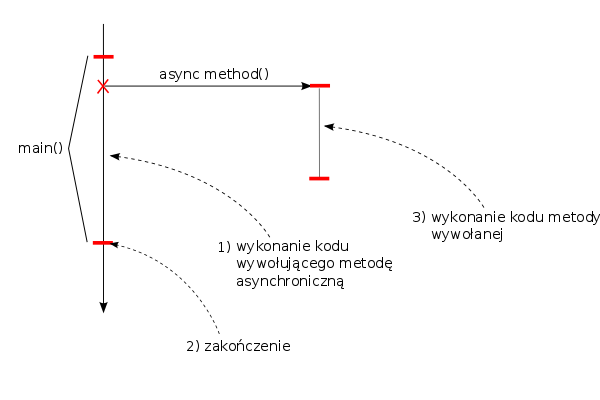
\includegraphics[scale=0.5]{figures/Rysunek5.png}
\end{figure}
}

\subsection{Blokowanie wywołań}
\begin{frame}[fragile]
\frametitle{Blokowanie wywołań}
\begin{block}{\texttt{BlockUntil(bool condition)}}  
Jeśli \texttt{condition = true}, to nic się nie dzieje (kontynuacja przetwarzania).  

W przeciwnym wypadku wycofanie aktualnej transakcji i ponowna próba po pewnym czasie.
\end{block}  

\vspace{20px}

\begin{alertblock}{Ważne!}
Jeśli metoda asynchroniczna (transakcja) zatrzyma się na którejś z kolei instrukcji \texttt{BlockUntil()}, wycofywana jest cała transakcja!
\end{alertblock}
\end{frame}

\frame{\frametitle{Blokowanie wywołań}
\begin{figure}[h]
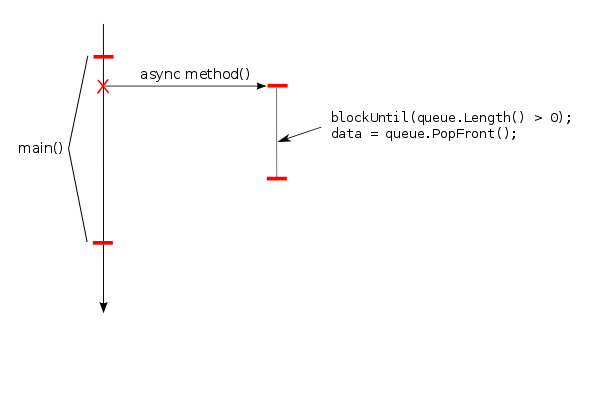
\includegraphics[scale=0.5]{figures/Rysunek6.png}
\end{figure}
}

\subsection{Przykład}
\begin{frame}[fragile]
\frametitle{Przykład Zombie}
\begin{columns}
	\begin{column}{0.35\paperwidth}
		{\scriptsize\begin{verbatim}
			void startZombie() {
			    Zombie z;
			    z.initialize();
			    async UpdateZombie(z);
			}
		\end{verbatim}}
	\end{column}  
	\begin{column}{0.55\paperwidth} 
		{\scriptsize\begin{verbatim}
			void UpdateZombie(Zombie z) {
			    Time now = GetTimeNow();
			    BlockUntil(now - z.lastUpdate >
			            z.updateInterval);
			    z.lastUpdate = now;
			    MoveAround(z);
			    if (Distance(z, player) < DeathRadius) {
			        KillPlayer();
			    } else {
			        async UpdateZombie(z);
			    }
			}
		\end{verbatim}}
	\end{column}
\end{columns}
\end{frame}

\section{Szczegółowy model}
\frame{\frametitle{}
\begin{center}
	\Large{\textbf{SZCZEGÓŁOWY MODEL \\ SYSTEMU AME}}
\end{center}
}

\subsection{Dzielenie metod}
\frame{\frametitle{I co dalej?}
\begin{block}{Problem}
Długie metody z wieloma instrukcjami \texttt{BlockUntil()} będą częściej powodować wycofanie transakcji.
\end{block}  

\vspace{15px}

\begin{exampleblock}{Rozwiązanie}
Podział aktualnej transakcji za pomocą metody \texttt{Yield()} na atomowe bloki.   

\vspace{5px}

\texttt{BlockUntil()} zablokuje tylko fragment od poprzedniego wywołania metody \texttt{Yield()}, a jeśli będzie wznawiać działanie po aborcie, zrobi to od poprzedniego wywołania \texttt{Yield()}.
\end{exampleblock}
}

\frame{\frametitle{Używanie \texttt{Yield()}}
Wymagane jest, aby metoda zawierająca \texttt{Yield()} deklarowała w swoim nagłówku słowo kluczowe \texttt{yields}:
\begin{block}{}
\texttt{returnType someMethod(args) yields \{ ... \} }
\end{block}
\vspace{15px}
Natomiast każde wywołanie metody zawierającej \texttt{Yield()} powinno wyglądać następująco:
\begin{block}{}
\texttt{int foo = someMethod(x) yielding;} 
\end{block}
} 

\frame{\frametitle{Dzielenie metod -- przykład}
\begin{figure}[h] 
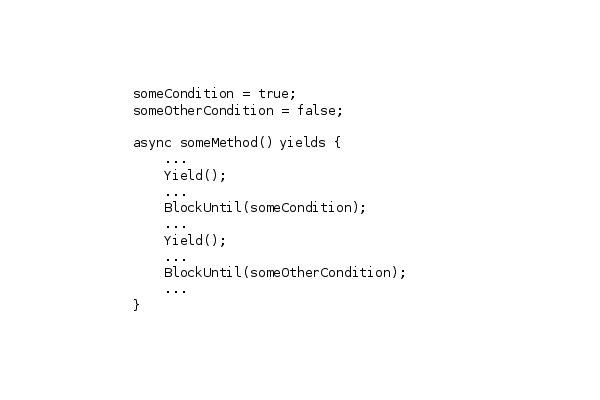
\includegraphics[scale=0.5]{figures/Rysunek10.png}
\end{figure}
}

\frame{\frametitle{Dzielenie metod -- przykład}
\begin{figure}[h] 
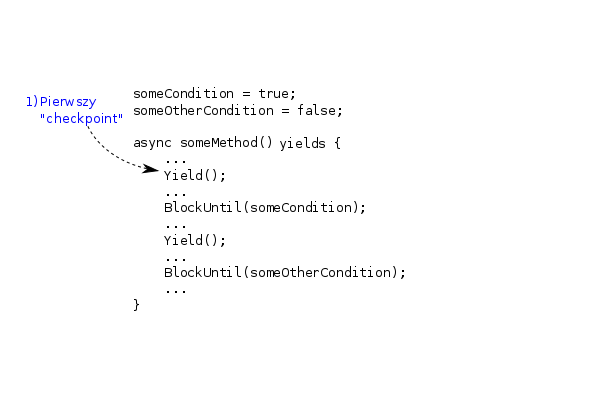
\includegraphics[scale=0.5]{figures/Rysunek11.png}
\end{figure}
}

\frame{\frametitle{Dzielenie metod -- przykład}
\begin{figure}[h] 
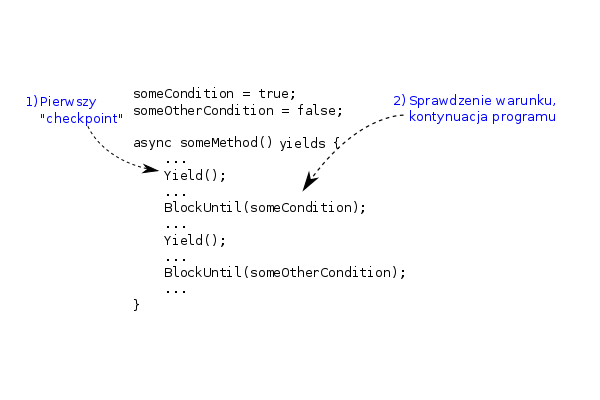
\includegraphics[scale=0.5]{figures/Rysunek12.png} 
\end{figure}
}

\frame{\frametitle{Dzielenie metod -- przykład}
\begin{figure}[h] 
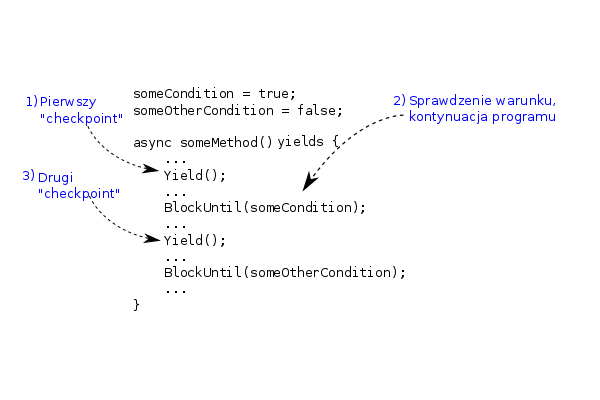
\includegraphics[scale=0.5]{figures/Rysunek13.png}
\end{figure}
}

\frame{\frametitle{Dzielenie metod -- przykład}
\begin{figure}[h] 
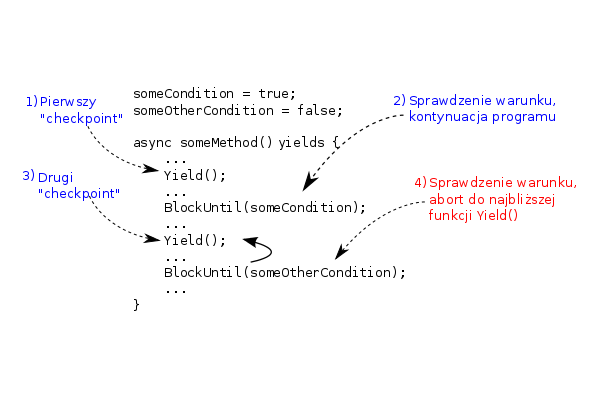
\includegraphics[scale=0.5]{figures/Rysunek14.png}
\end{figure}
}


\begin{frame}[fragile]
\frametitle{Dzielenie metod -- przykład Zombie}
\begin{columns}
	\begin{column}{0.45\paperwidth} 
		{\fontsize{7pt}{8pt}
			\begin{verbatim}
			void startZombie() {
			    Zombie z;
			    z.initialize();
			    async UpdateZombie(z);
			}
			
		\end{verbatim}
		}
		{\fontsize{7pt}{8pt}
		\begin{verbatim}
			void UpdateZombie(Zombie z) {
			    Time now = GetTimeNow();
			    BlockUntil(now - z.lastUpdate >
			            z.updateInterval);
			    z.lastUpdate = now;
			    MoveAround(z);
			    if (Distance(z, player) < DeathRadius) {
			        KillPlayer();
			    } else {
			        async UpdateZombie(z);
			    }
			}
		\end{verbatim}}
	\end{column}  
	\begin{column}{0.45\paperwidth} 
		{\fontsize{7pt}{8pt}\begin{verbatim}
			void RunZombie() yields {
			    Zombie z;
			    z.initialize();
			    while (Distance(z, player) >= 
			           DeathRadius) {
			        Yield();
			        Time now = GetTimeNow();
			        BlockUntil(now - z.lastUpdate > 
			                   z.updateInterval);
			        z.lastUpdate = now;
			        MoveAround(z);
			        if (Distance(z, player) < 
			            DeathRadius) {
			            KillPlayer(); 
			        }
			    }
			}
		\end{verbatim}}
	\end{column}
\end{columns}
\end{frame}

\subsection{Niesynchronizowany kod}
\frame{\frametitle{\texttt{unprotected \{ ... \}}}
\begin{block}{}
Użycie bloku \texttt{unprotected} powoduje zakończenie aktualnej transakcji (commit/yield), następnie wykonanie kodu wewnątrz bloku bez synchronizacji i rozpoczęcie nowej transakcji
\end{block} 
\vspace{15px}  
\begin{block}{}
Każda metoda korzystająca z \texttt{unprotected} musi mieć w nagłówku słowo kluczowe \texttt{yields}.
\end{block}
}

\begin{frame}[fragile]
\frametitle{\texttt{unprotected \{ ... \}}}
\begin{verbatim}
void method yields {
    << someCode1 >>
    ...
    unprotected {             // end of transaction
        unsynchronizedCode
    }                         // start of new transaction
    ...
    << someCode2 >>
}
\end{verbatim}
\end{frame}

\section{Zakończenie}
\subsection{Podsumowanie}
\frame{\frametitle{Podsumowanie}
\begin{block}{}
\textit{We encourage correctness first, performance second and maintainability always.}
\end{block}
\vspace{10px}  
\begin{block}{}
System oparty zarówno na transakcjach jak i standardowych mutexach.
\end{block}
\vspace{10px}  
\begin{block}{}
Przemyślany dla utrzymania systemów dużych i żywotnych.
\end{block}
}

\subsection{Wyzwania}
\frame{\frametitle{Wyzwania}
\begin{block}{}
Scheduling w celu zminimalizowania ilości cofniętych transakcji.
\end{block} 
\vspace{10px}  
\begin{block}{}
Optymalizacje sytuacji, gdy \texttt{BlockUntil} stoi na początku fragmentu atomowego.
\end{block} 
\vspace{10px}  
\begin{block}{}
Wzbogacenie instrukcji \texttt{Yield} np. o deklarowanie zmiennych uaktualnianych tą funkcją, dzięki czemu wzrośnie poprawność.
\end{block}
}

\frame{\frametitle{Dziękuję za uwagę}
\begin{center}
\Large{\textbf{DZIĘKUJĘ ZA UWAGĘ}}

\vspace{10px}
\large{Filip Rachwalak}
\end{center}
}

\end{document}